% This is samplepaper.tex, a sample chapter demonstrating the
% LLNCS macro package for Springer Computer Science proceedings;
% Version 2.20 of 2017/10/04
%
\documentclass[runningheads]{llncs}
%
\usepackage{graphicx}
\usepackage{lipsum}
\usepackage{kotex}
\usepackage{url}
\usepackage{indentfirst}
\usepackage{bibentry}
\usepackage{wrapfig}

% \bibliographystyle{plainnat}
\nobibliography*
\bibliographystyle{splncs04}
% Used for displaying a sample figure. If possible, figure files should
% be included in EPS format.
%
% If you use the hyperref package, please uncomment the following line
% to display URLs in blue roman font according to Springer's eBook style:
% \renewcommand\UrlFont{\color{blue}\rmfamily}

\begin{document}
%
\title{Stock Price Prediction System\thanks{Supported by LINC}}
%
%\titlerunning{Abbreviated paper title}
% If the paper title is too long for the running head, you can set
% an abbreviated paper title here
%
\author{Chanyoung Lee\inst{1}{2019313902} \and
Yujin Seo\inst{2}{2018314589} \and
Donghun Jung\inst{3}{2020312141}}
%
% \authorrunning{F. Author et al.}
% First names are abbreviated in the running head.
% If there are more than two authors, 'et al.' is used.
%
\institute{
Sungkyunkwan University, Computer Science and Engineering, Republic of Korea \and
Sungkyunkwan University, Department of Mathematics, Republic of Korea \and
Sungkyunkwan University, Department of Physcis, Republic of Korea 
% Springer Heidelberg, Tiergartenstr. 17, 69121 Heidelberg, Germany
% \email{lncs@springer.com}\\
% \url{http://www.springer.com/gp/computer-science/lncs} \and
% ABC Institute, Rupert-Karls-University Heidelberg, Heidelberg, Germany\\
% \email{\{abc,lncs\}@uni-heidelberg.de}
}
%
\maketitle              % typeset the header of the contribution
%
\begin{abstract}
This project aims to predict the stock price of some selected stocks in KODEX 200 and S\&P 500 on a day-by-day basis.
Leveraging data sourced from the Korea Exchange (KRX) and Nasdaq, we will undertake the training and evaluation of a diverse set of machine learning models, including Long Short-Term Memory (LSTM), Gated Recurrent Unit (GRU), and Transformer. 
We focus on predicting the stock price of the next day. 
In a contrast to the general stock price prediction system of many stock firms, we do not analyse the fundamental of the company. 
We focus on the short-term changes of the stock price, and attempts to reflect the recent issues via VADER.



% This accessibility contributes significantly to
% the domains of investment decision-making, lowering the entry barrier for
% users interested in this field. Given the computationally intensive nature
% of our endeavor, our primary focus remains on constructing an accurate
% predictive model specifically designed for the stock prices of SAMSUNG
% Electronics. SAMSUNG Electronics stands as one of the most popular
% and actively traded stocks in South Korea, making it an ideal candidate
% for our predictive model. Furthermore, as a testament to our commitment
% to accessibility, our model will be deployed as a publicly accessible web
% service. This ensures that users can harness the power of our predictive
% model conveniently.
\keywords{Stock Price Prediction \and Machine Learning \and LSTM \and GRU \and Transformer \and VADER}

\end{abstract}
%
%
%
\section{Introduction}
\label{sec:Introduction}
In today's capitalist world, stocks present an attractive avenue for financial gain, offering significant profit potential. 
Investors, regardless of their depth of understanding of the stock market, are constantly seeking reliable methods to predict future stock prices, as their financial well-being often hinges on these predictions.

Predicting stock prices is fundamentally about discerning the real value of a company. 
Knowing a company's true value helps in determining whether its stock price will rise or fall from its current level. 
However, this is a complex task influenced by a myriad of factors, including global events and economic conditions.

Historically, professional fund managers have been pivotal in guiding investments in the stock market. 
However, their strategies and predictions are susceptible to personal biases. 
This limitation has spurred interest in leveraging machine learning for more objective and unbiased stock price forecasting.

While numerous services today use machine learning for this purpose, many are not open-source and are primarily geared towards professional investors. 
These systems, often complex and tailored for experienced users, focus more on asset allocation than on precise stock price prediction. 
In contrast, our project targets the general public, who rely more on simple chart analysis and intuition, without delving deep into a company's fundamentals or news events.

Our proposal is to predict the short-term movement of blue-chip stocks, a strategy known to be effective over periods ranging from a few days to a few months. 
We aim to make short-term predictions, not in real-time, to assist general users and simplify the prediction process.

To achieve this, we have employed machine learning techniques, utilizing models such as Long Short-Term Memory(LSTM), Gated Recurrent Unit(GRU), and Transformer. 
These models have been instrumental in successfully predicting stock prices for the next few days by capturing short-term trends. 
In addition, we have integrated VADER, a sentiment analysis tool, to reflect recent issues and capture both short- and long-term stock price changes based on current events.

Our system has been deployed as a publicly accessible web service, offering users easy access to our predictive model. 
This deployment significantly contributes to investment decision-making, lowering the entry barrier for those interested in stock market investments. 
Empirical evaluations of our system have shown promising results in capturing short-term trend of stock price movements, thereby validating our approach and offering a valuable tool for investors.

\section{Background and Related Works}
\label{sec:BackgroundAndRelatedWorks}
\subsection{Background and Related Works}

\subsubsection{Stock Price Prediction}
Stock Price Prediction is the task of forecasting future stock prices based on historical data and various market indicators. 
It involves the use of statistical models and machine learning algorithms to analyze financial data and make predictions about a stock's future performance. 
Stock price trends are influenced by numerous factors, including interest rates, inflation rates, and financial news. 
To make accurate stock price predictions, one must leverage this diverse set of information. 
In the banking industry and financial services sector, teams of analysts are dedicated to scrutinizing, analyzing, and quantifying qualitative data from news sources. 
A substantial amount of information regarding stock trends is extracted from the extensive corpus of textual and quantitative data involved in such analysis.

\subsubsection{Research Trends}
Recent research trends in stock price prediction include advancements in deep learning-based regression models. 
These models often utilize Long Short-Term Memory (LSTM) networks and innovative validation techniques, such as walk-forward validation, to enhance their predictive capabilities.

In addition, some researchers have explored Particle Filter Recurrent Neural Networks (PF-RNNs), a new RNN family explicitly designed to model uncertainty within their internal structure. 
Unlike traditional RNNs that rely on a deterministic latent state vector, PF-RNNs maintain a latent state distribution approximated as a set of particles. 
To enable effective learning, researchers have introduced a fully differentiable particle filter algorithm that updates the PF-RNN latent state distribution based on Bayes' rule. 
Experimental results have shown that PF-RNNs can outperform conventional gated RNNs across various domains, 
including synthetic robot localization datasets and real-world sequence prediction tasks, which is stock price prediction.

Furthermore, recent studies have proposed novel approaches, such as the development of a sentiment-ARMA model, which combines the autoregressive moving average model (ARMA) with sentiment analysis of financial news articles. 
This model is integrated into an LSTM-based deep neural network consisting of three components: LSTM, VADER model, and a differential privacy (DP) mechanism. 
The proposed DP-LSTM scheme has demonstrated the potential to reduce prediction errors and enhance model robustness. Extensive experiments conducted on S\&P 500 stocks have indicated promising results, 
including a 0.32\% improvement in mean Mean Percentage Absolute Error (MPA) 
and a significant up to 65.79\% reduction in Mean Squared Error (MSE) for the prediction of the market index S\&P 500.

% \subsection{Background and Related Works}

% \subsubsection{Stock price prediction}
% Stock Price Prediction is the task of forecasting future stock prices based on historical data and various market indicators. 
% It involves using statistical models and machine learning algorithms to analyze financial data and make predictions about the future performance of a stock. 
% Stocks' trends are affected by a lot of factors such as interest rates, inflation rates and financial news.
% To predict stock prices accurately, one must use these variable information. In particular, in the
% banking industry and financial services, analysts' armies are dedicated to pouring over, analyzing,
% and attempting to quantify qualitative data from news. A large amount of stock trend information is
% extracted from the large amount of text and quantitative information that is involved in the analysis.

% \subsubsection{Research trend}
% We, then, augment the
% predictive power of our forecasting framework by building four deep learning-
% based regression models using long-and short-term memory (LSTM) networks
% with a novel approach of walk-forward validation.

% Particle Filter Recurrent Neural Networks (PF-RNNs),
% a new RNN family that explicitly models uncertainty in its in-
% ternal structure: while an RNN relies on a long, deterministic
% latent state vector, a PF-RNN maintains a latent state distribu-
% tion, approximated as a set of particles. For effective learning,
% we provide a fully differentiable particle filter algorithm that
% updates the PF-RNN latent state distribution according to the
% Bayes rule. Experiments demonstrate that the proposed PF-
% RNNs outperform the corresponding standard gated RNNs
% on a synthetic robot localization dataset and 10 real-world se-
% quence prediction datasets for text classification, stock price
% prediction, etc.

% First, based on the autoregressive moving average model (ARMA), a sentiment-
% ARMA is formulated by taking into consideration the information of financial
% news articles in the model. Then, an LSTM-based deep neural network is designed,
% which consists of three components: LSTM, VADER model and differential privacy
% (DP) mechanism. The proposed DP-LSTM scheme can reduce prediction errors
% and increase the robustness. Extensive experiments on S&P 500 stocks show that (i)
% the proposed DP-LSTM achieves 0.32\% improvement in mean MPA of prediction
% result, and (ii) for the prediction of the market index S&P 500, we achieve up to
% 65.79\% improvement in MSE.	





% https://paperswithcode.com/task/stock-price-prediction 
% 사이트를 참고하였습니다

% https://arxiv.org/ftp/arxiv/papers/2009/2009.10819.pdf
% LSTM을 이용하여 일일 단위 고가/저가를 예측한 모델입니다. 데이터 구성에는 일일 단위로 시가, 고가, 저가 , 종가, 거래량이 있네요. LSTM 모델 구현할 때 참고할 만 합니다.

% https://arxiv.org/pdf/1905.12885v2.pdf
% Particle Filtering을 적용한 LSTM과 GRU에 대해 설명하는 논문입니다. Particle Filtering은 비가우시안 통계를 따르는 데이터를 가우시안 통계로 근사하는 알고리즘인 것으로 이해했는데, 이를 적용하면 sequence 예측 성능이 개선되는 것 같아 고려할만한 LSTM과 GRU모델이 될 것 같습니다.

% https://arxiv.org/pdf/1912.10806v1.pdf
% 예측 모델로는 ARMA모델을 사용했는데, Sentiment Analysis 부분에서 참고할만한 내용이 있어서 선정하게 되었습니다. Sentiment Analysis 부분에서는 VADER를 사용했는데, 기업 공시 혹은 뉴스 정보도 예측에 사용한다면 도움이 될 것 같습니다.
% VADER 모델은 Sentiment Analysis을 수행하는 NLP모델입니다. 사전 학습이 되어 있어 따로 학습시킬 필요 없이 바로 사용할 수 있고, VADER 출력에 대해 적절히 임베딩만 해준다면 사용하기 간편할 것 같습니다.

% (논문이 거의 다 LSTM 뿐이네요... GRU도 조금만 보이고, CNN과 Transformer는 찾아볼 수 없었습니다ㅠㅠ 근데 우선 저정도로 하면 학습 방식 혹은 감성 분석 시 적용할 기술에 대해서는 참고할 양이 충분한 것 같습니다)

\section{Problem Statement and Proposed Solution}
\label{sec:ProblemStatementAndProposedSolution}
\subsection{Problem Statement}



\subsection{Proposed Solutions}
\subsubsection{LSTM}
Long Short-Term Memory(LSTM) is an advanced Recurrent Neural Network (RNN) architecture 
as shown in the Figure. 
LSTMs were introduced to address some of the limitations of traditional RNNs, 
which struggle with capturing long-range dependencies in sequential data due to the vanishing gradient problem.

LSTM has three gates: input gate, forget gate, and output gate.
\begin{enumerate}
	\item Input gate: 	Input gate is denoted by orange box. It decides what new information should be stored in the cell.
	\item Forget gate:	Forget gate is denoted by blue box. It determines what information from the previous state should be discarded or reflected.
	\item Output gate:	Output gate is denoted by gray box. The actual outputs are $h_{i}$ and $y_{i}$, which are same and $c_{i}$ represents the status of the cell. It specifies what information from the cell should be used to generate the output.
\end{enumerate}

Compared to the traditional RNN, LSTM performs various mathematical operations, including including element-wise multiplication and addition, to control the flow of information and perform updates to the memory cell and hidden state.

Through this architecture and characteristics, LSTM can handle the long sequential data by maintaining a memory cell with gates to control information flow, 
making it capable of capturing long-term dependencies and patterns in the data.

\subsubsection{GRU}

A Gated Recurrent Unit(GRU) is another type of recurrent neural network (RNN) architecture, 
similar to the Long Short-Term Memory (LSTM) network. 
GRUs are simpler in structure compared to LSTMs but have been found to be highly effective in various applications. 
GRU is also designed to address the vanishing gradient problem and enable RNNs to better capture long-range dependencies in sequential data. 
Compared to LSTM, GRU does not distinguish between cell status and the output.

% Input gate, forget gate?
GRU has two gates: reset gate and update gate.
\begin{enumerate}
	\item Reset gate: Reset gate is denoted by color box. It decides how much of the past information to forget.
	\item Update gate: Update gate is denoted by color box. It decides how much of the past information to remember.
\end{enumerate}

GRUs also perform mathematical operations, including element-wise multiplications and additions, to control the flow of information and update the hidden state.

Through this architecture and characteristics, GRU can also handle the long sequential data by maintaining a memory cell with gates to control information flow, 
making it capable of capturing long-term dependencies and patterns in the data.


\subsubsection{One-dimensional CNN}

A Convolutional Neural Network(CNN) is a neural network architecture widely employed for processing and analyzing one-dimensional data sequences. 
In the context of stock price prediction, which inherently involves one-dimensional data, the utilization of a one-dimensional CNN is particularly relevant and effective.

Compared to other recurrent neural network (RNN) variants like LSTM and GRU, CNNs offer a notably simpler structural design. 
Also it seems possible to analyse the various patterns of stock price data through the convolutional layers.
As the stock price data is characterized by its non-stationary nature, exhibiting evolving trends and patterns over time, 
it is probable that CNN excels the performance of LSTM, and GRU.

\subsubsection{Transformer}



\section{Planning in Detail}
\label{sec:PlanningInDetail}
\subsection{Roles}

Our team is organized as follows: 
Donghun Jung serves as the team leader and is responsible for the development of the web front end.
Chanyoung Lee and Yujin Seo share responsibilities for developing the back end and the AI model.

\subsection{Tentative Schedule}
\begin{figure}[h]
	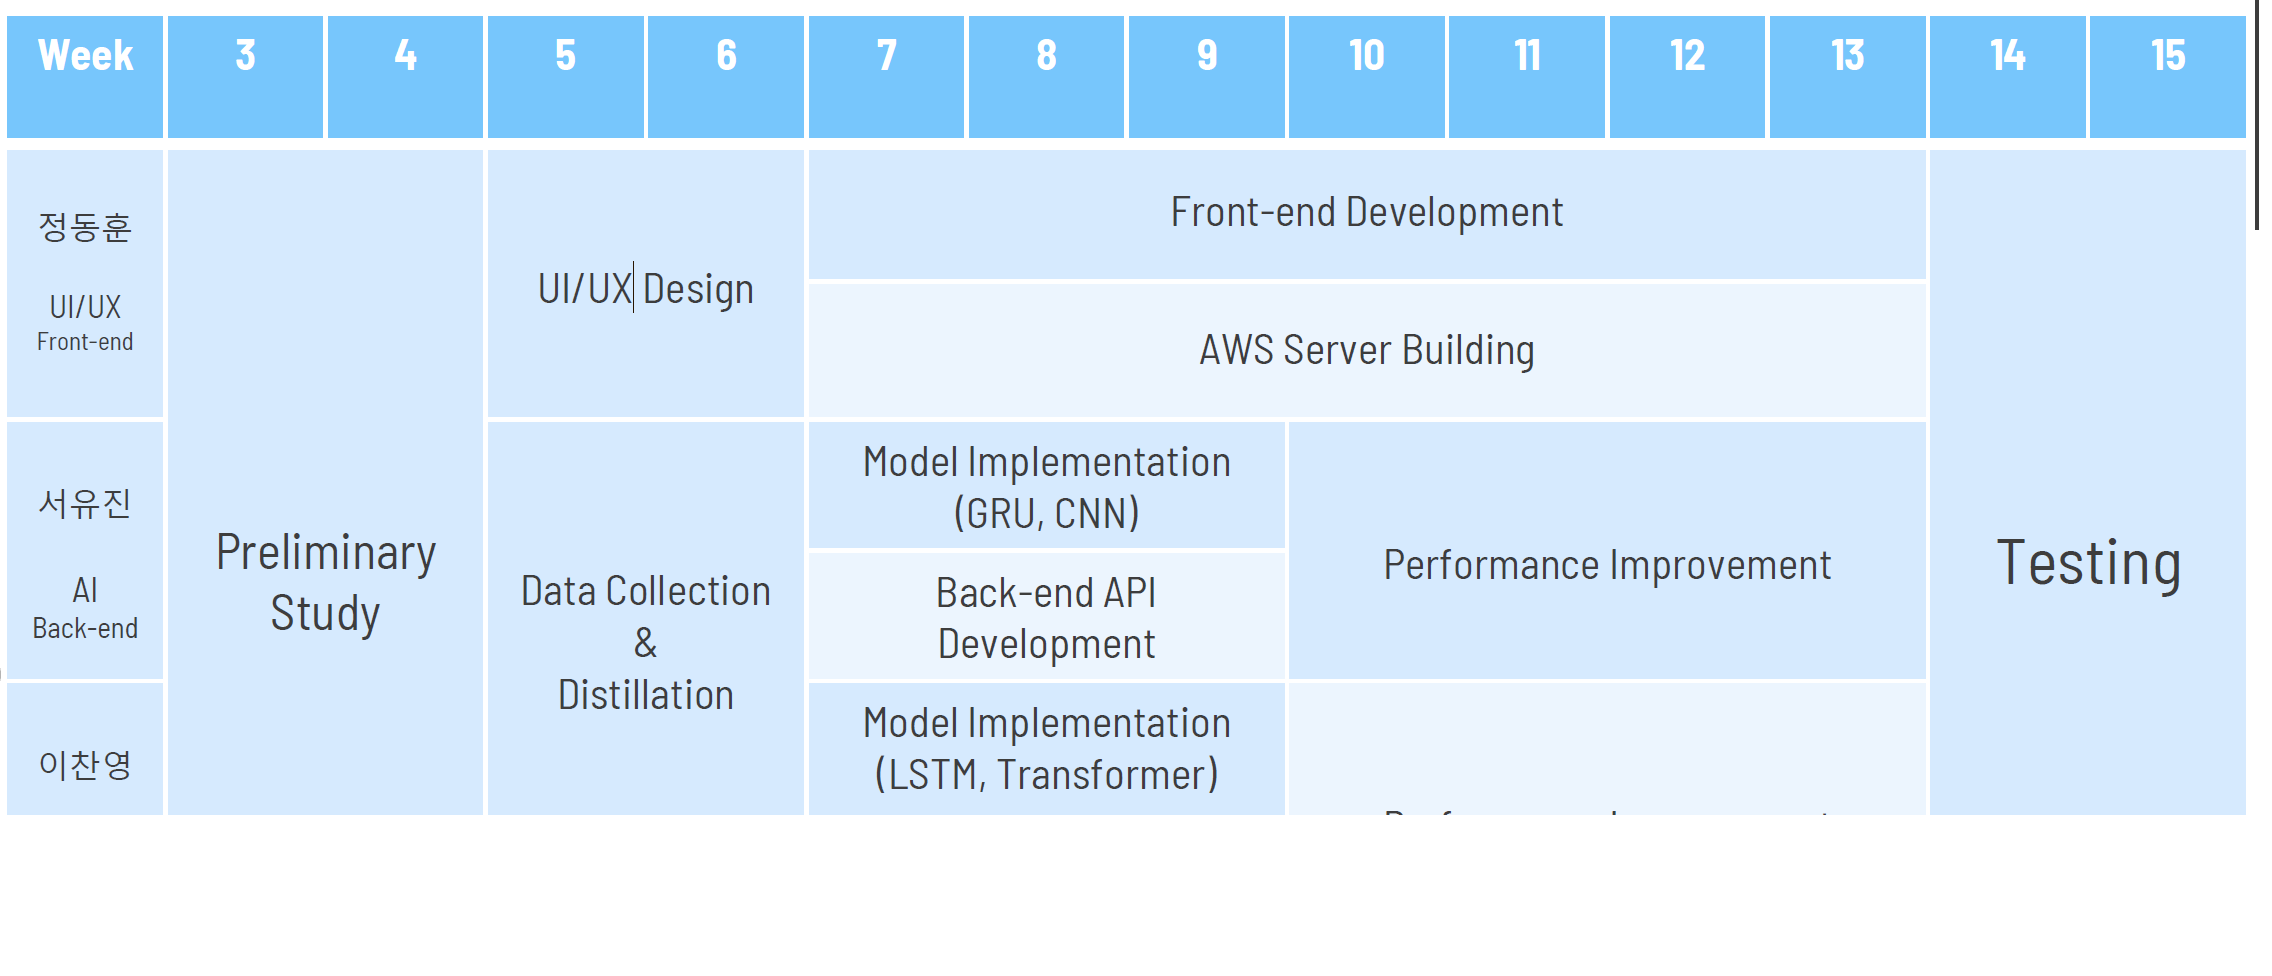
\includegraphics[width=\textwidth]{Fig/Schedule.png}
\end{figure}
Our project timeline is outlined as follows: 
In the first three weeks, we conducted preliminary studies and research to establish the project's foundation. 
From the fourth to the sixth week, the frontend team will focus on designing the user interface(UI) and user experience(UX), 
while the backend team will collect data and prepare the necessary infrastructure. 
In the subsequent weeks up to the thirteenth week, the frontend team will proceed to develop the web page and set up the AWS server, 
while the backend team will be responsible for implementing the AI model, designing backend APIs, and continually improving the model's performance. 
Finally, in the last three weeks leading up to the presentation, we will rigorously test the AI model and the web application before deploying the web page for the final presentation.


\bibliography{reference}

\end{document}
